\section{Dynamic Programming}

Two things that are needed for Dynamic Programming:\\

\emph{Optimal Substructure:} If an optimal solution to the problem can be constructed from optimal solutions to subproblems.\\

\emph{Overlapping Subproblems:} When a recursive algorith revisits the same problem repeatedly we say it has overlapping subproblems.\\

Divide and Conquer is not suited for problems that occur several times as this means it solves those \emph{overlapping subproblems} each time and dynamic program is a strategy to not have to recompute these problems. 

There are two main strategies of Dynamic programming.\\

\emph{Memoisation:} This strategy that is top-down idea that saves the solution to a subproblem in a data structure, and that then check up that value when you come acrosse the same subproblem again. \\

\emph{Iterative: } This is a bottom-up strategy 

\subsection{0/1 Knapsack Problem}

The 0/1 Knapsack problem is if a single object of weight and price should be included in the knapsack that can only carry a certain weight. The goal is to maximize the profit. \\

Given a price vector $p = {1, 2, 5, 6}$ and a weight vector $w = {2, 3, 4, 5}$. The solution to the problem is an vector that is binary indicating whether the object is included or not, $x = {0, 1, 0, 1}$. 
Since every item is either included or not, and all solution have to be checked the problem is $\mathcal{O}(2^n)$. This can be shortend by dynamic programming.\\

You set up a table where the columns is every weight that can be had in the bag. feks 1 - 8 for a bag that can take 8 kg. The row values are the objects in addition to having nothing in the bag. Since we are solving the problem for each step, there is a smell of optimal substructure and overlapping subproblems. 

The algorithm for this might be sligtly confusing, but just thing logically about the table. Fill the weight for each of these and put in the next object for the next weight.

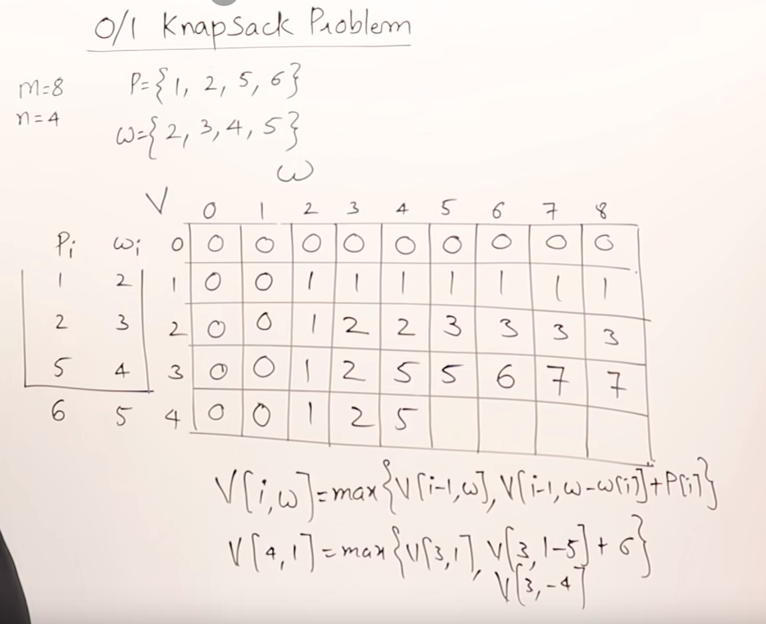
\includegraphics[width=\textwidth]{images/01Knapsack.png}

\subsection{Rod cutting}

Rod cutting problem is determining the optimal number of cuts to be done a rod. There are different prices for different lengths of the rod. You would have a length of the rod and a corresponding price $p = {1, 5, 8, 9, 10, 17, 17, 20}$. The idea is to solve the problem for each lengths $i$ of the rod and a corresponding \emph{optimal price} vector. The algorithm uses the following  to solve the problem. 

\begin{equation}
    C(i)=\max_{1\leq k \leq i}\{V_k + C(i-k)\}
\end{equation}

Where $C(i)$ is the optimal cost at index $i$, and $k$ is the number of cuts\, 
This essentially means taking the maximum previous ($C(i-k)$) and adding on the price, based on the length left over based on he price ($5$). This uses the table below and previously calculated problems to find the optimal solution. 

Without dynamic programming this problem has a solution of $\mathcal{O}(2^n)$, but with dynamic programming it reduces to $\mathcal{O}(n^2)$,

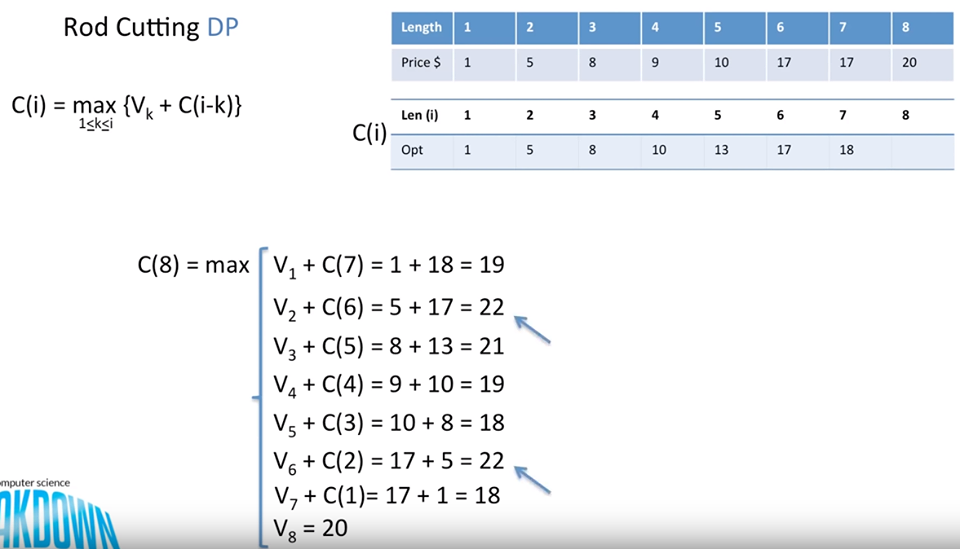
\includegraphics[width=\textwidth]{images/RodCutting.png}

\section{Greedy Programming}

There are two requirements for greedy programming:

\emph{The Greedy Choice Property} is that a global optimal solution can be arrived at by selecting a local optimmum.\\

\emph{Optimal Substructure:} If an optimal solution to the problem can be constructed from optimal solutions to subproblems.\\

\subsection{Activity Selection}

This is the problem is to choose as many activity as possible that do not overlap. In this type of problem the optimal solution is the always take the activity that finishes first relative to the ending time of the last activity. Therefore the problem is an example of a use of a greedy algorithm. 

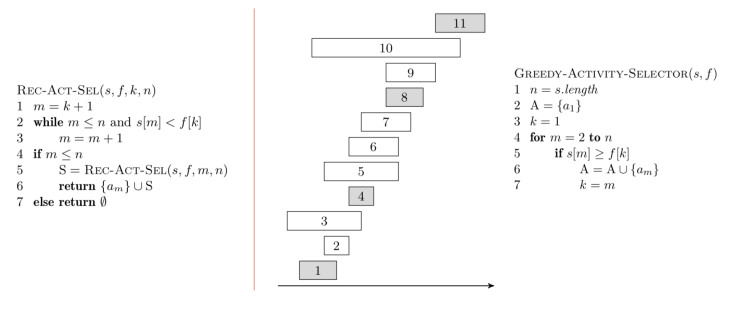
\includegraphics[width=\textwidth]{images/ActivitySelection.png}

\subsection{Huffman Coding Algorithm}

This is a compression algorithm that uses greedy programming. Remember information flow from TilpDat. 
The ideas is that you try to minimize the code, by assigning less bits to the symbol that occurs the most and more bits for those that occur less often. 

\begin{enumerate}
    \item The first step of the algorithm is to take the two characters with the lowest frequency.
    \item Then make a subtree from them and write the sum of the frequencies of both letters in the node above them.
    \item Now take the next lowest occurring symbol and set it beside the previous parent node and create a new parent node from the two. 
    \item Label the parent node with the total number of occurences in the new tree.
    \item Continue iterating through this method until the current parent node is greater than the frequency of all other nodes. 
    \item When this occurs, you need to start a new subtree with the remaining lowest frequency letters and create a parent node like we initially did.
    \item If there are remaining letters you want to take the lowest value subtree and lowest value letter and attach them together. 
    \item Finally, attach the subtrees together.
\end{enumerate}

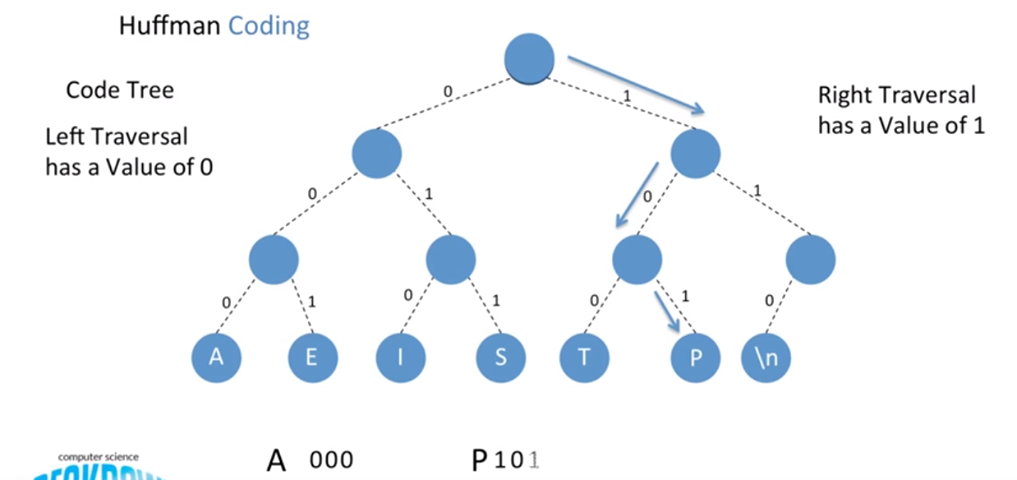
\includegraphics[width=\textwidth]{images/NonHuffman.png}

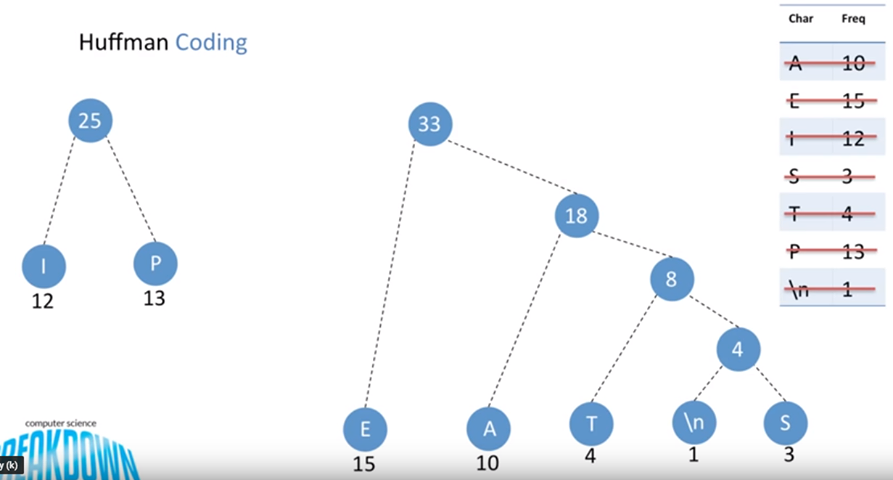
\includegraphics[width=\textwidth]{images/Huffman.png}